\documentclass{article}
\usepackage[paperwidth=275mm,paperheight=205mm,margin=0pt]{geometry}
\usepackage{tikz}
\usepackage{graphicx}
\usepackage{amsmath,amssymb}
\usepackage{xcolor}
\graphicspath{{report/image/}{image/}}
\usetikzlibrary{arrows.meta,backgrounds,calc,fit,positioning}
\pagestyle{empty}

% Paper-oriented palette: role is still identifiable in grayscale.
\definecolor{panel}{HTML}{FFFFFF}
\definecolor{ink}{HTML}{30343B}
\definecolor{targetgray}{HTML}{777B82}
\definecolor{encoderfill}{HTML}{E8E1F0}
\definecolor{modelfill}{HTML}{F3DCCF}
\definecolor{decoderfill}{HTML}{F3E2A9}
\definecolor{bodyfill}{HTML}{DDEED6}
\definecolor{latentfill}{HTML}{E4F3FA}
\definecolor{latentblue}{HTML}{5AA9CE}
\definecolor{featureblue}{HTML}{5B8FD9}
\definecolor{lossfill}{HTML}{FFFFFF}
\definecolor{emphasisred}{HTML}{D94A45}

\tikzset{
  font=\sffamily\footnotesize,
  >={Latex[length=2.2mm,width=1.4mm]},
  flow/.style={draw=ink, line width=.85pt, ->},
  line/.style={draw=ink, line width=.85pt},
  clearflow/.style={draw=ink, line width=.9pt, ->,
    preaction={draw=panel, line width=3.2pt}},
  clearline/.style={draw=ink, line width=.9pt,
    preaction={draw=panel, line width=3.2pt}},
  target/.style={draw=targetgray, line width=.75pt, dashed, ->},
  operation/.style={draw=ink!75, fill=white, line width=.65pt,
    rounded corners=1.5pt, align=center, minimum width=13mm,
    minimum height=5.5mm, inner sep=1.5pt, font=\sffamily\scriptsize},
  encoder/.style={draw=ink!75, fill=encoderfill, line width=.7pt,
    rounded corners=2pt, align=center, minimum width=19mm,
    minimum height=12mm, inner sep=2.5pt},
  model/.style={draw=ink, fill=modelfill, line width=.8pt,
    rounded corners=2.5pt, align=center, minimum width=32mm,
    minimum height=10mm, inner sep=3pt},
  decoder/.style={model, fill=decoderfill, minimum width=29mm, minimum height=10mm},
  bodyhead/.style={model, fill=bodyfill, minimum width=32mm, minimum height=10mm},
  latent/.style={draw=latentblue, fill=latentfill, line width=1.2pt,
    rounded corners=3pt, align=center, minimum width=17mm,
    minimum height=10mm, inner sep=1.5pt,
    font=\sffamily\bfseries\footnotesize},
  loss/.style={draw=ink!80, fill=lossfill, line width=.75pt,
    rounded corners=4pt, align=center, minimum width=18mm,
    minimum height=8mm, inner sep=1.8pt},
  hotmodel/.style={model, draw=emphasisred, line width=1.4pt},
  hotbodyhead/.style={bodyhead, draw=emphasisred, line width=1.4pt},
  hotloss/.style={loss, draw=emphasisred, line width=1.35pt},
  steptag/.style={circle, draw=ink, fill=ink, text=white,
    inner sep=0pt, minimum size=4.2mm,
    font=\sffamily\bfseries\tiny},
  imageframe/.style={draw=ink!65, fill=white, line width=.65pt,
    rounded corners=1pt, inner sep=0pt},
  hotimageframe/.style={draw=emphasisred, fill=white, line width=2.65pt,
    rounded corners=1pt, inner sep=0pt},
  junction/.style={circle, fill=ink, inner sep=0pt, minimum size=2mm},
  labelbox/.style={fill=panel, inner sep=1pt, font=\scriptsize}
}

\begin{document}
\thispagestyle{empty}
\vspace*{\fill}
\noindent\makebox[\paperwidth][c]{%
\begin{tikzpicture}[x=1mm,y=1mm]
  % One semantic region: only pretraining is shown in this figure.
  \begin{scope}[on background layer]
    \path[draw=ink!35, fill=panel, line width=.8pt, rounded corners=5pt]
      (-7,-47) rectangle (240,47);
  \end{scope}
  \node[font=\sffamily\bfseries\large, text=ink] at (117,41) {Pretraining};

  % -----------------------------------------------------------------------
  % Paired observations: visual objects rather than network-style boxes.
  \node[imageframe] (frameT) at (5.4,10.1)
    {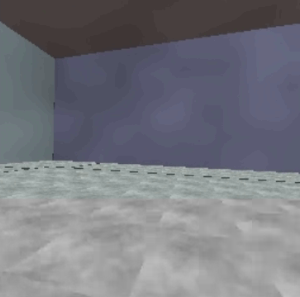
\includegraphics[width=20mm,height=14mm]{1.png}};
  \node[imageframe] (frameTp1) at (7.8,4.9)
    {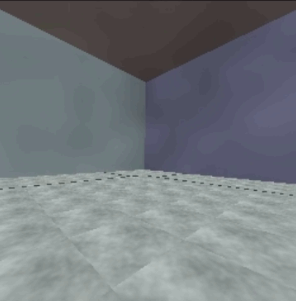
\includegraphics[width=20mm,height=14mm]{2.png}};
  \node[anchor=south east, font=\scriptsize] at (frameT.north east) {$o_t$};
  \node[anchor=south east, font=\scriptsize] at (frameTp1.north east) {$o_{t+1}$};
  \node[align=center, font=\scriptsize, text=ink!80] at (8,-7)
    {Adjacent RGB\\observations};

  % Synchronized action supervision is kept visually secondary.
  \node[align=center, font=\scriptsize, text=ink!85] (label)
    at (14,35) {Body-motion label\\$\mathbf v_t$};
  \node[align=center, font=\scriptsize, text=ink!85] (bodylabel)
    at (14,-35) {Joint-command label\\$a_t$};

  % -----------------------------------------------------------------------
  % Two independently augmented views.
  \coordinate (obsSplit) at (26,5);
  \draw[line] (frameTp1.east) -- (obsSplit);
  \node[junction] at (obsSplit) {};
  \node[operation] (augA) at (40,19) {Aug. $A$};
  \node[operation] (augB) at (40,-9) {Aug. $B$};
  \draw[flow] (obsSplit) |- (augA.west);
  \draw[flow] (obsSplit) |- (augB.west);

  % Two forward passes through one shared, frozen visual model.
  \node[encoder] (encA) at (63,19) {Frozen Visual\\Encoder};
  \node[encoder] (encB) at (63,-9) {Frozen Visual\\Encoder};
  \draw[flow] (augA) -- (encA);
  \draw[flow] (augB) -- (encB);
  % Feature-token glyphs distinguish data representations from computations.
  \foreach \dy/\h in {-3/7,-1/11,1/9,3/13} {
    \fill[featureblue!82] (79+\dy,19-\h/2) rectangle ++(1.7,\h);
    \fill[featureblue!82] (79+\dy,-9-\h/2) rectangle ++(1.7,\h);
  }
  \coordinate (featuresA) at (86,19);
  \coordinate (featuresB) at (86,-9);
  \node[align=center, labelbox] (featuresALabel) at (80,11.5)
    {$(e_t^{A},e_{t+1}^{A})$};
  \node[align=center, labelbox] (featuresBLabel) at (80,-17)
    {$(e_t^{B},e_{t+1}^{B})$};
  \draw[flow] (encA.east) -- (featuresA);
  \draw[flow] (encB.east) -- (featuresB);
  \node[draw=ink!28, dashed, rounded corners=3pt,
    fit=(augA)(augB)(encA)(encB)(featuresALabel)(featuresBLabel), inner sep=4pt,
    label={[font=\scriptsize,text=ink!62]below:visual front-end; shared frozen encoder}]
    (visualfrontend) {};

  % -----------------------------------------------------------------------
  % The ITM produces one latent vector.  A small circular data node keeps it
  % visually distinct from the learned modules that compute with it.
  \node[model] (itm) at (112,19)
    {Inverse Transition Model};
  \draw[flow] (featuresA) -- (itm.west);

\node[latent] (z) at (140,1)
  {$z_t $\hspace{1.0mm}{\scriptsize\color{latentblue!85!black}$\in \mathbb{R}^{64}$}};
\node[font=\scriptsize, text=ink!75, above=2.0mm of z]
  {latent action};
  
  \draw[clearflow] (itm.south) -- (112,1) -- (z.west);

  \node[bodyhead] (bodyhead) at (180,21)
    {Body-motion Head};
  \node[model] (ftm) at (180,1)
    {Forward Transition Model};
  \node[decoder] (md) at (180,-23)
    {Motion Decoder};
  \draw[clearflow] (z.north) -- (140,21) -- (bodyhead.west);
  \draw[clearflow] (z.east) -- (ftm.west);
  \draw[clearflow] (z.south) -- (140,-20.2) -- ($(md.west)+(0,2.8)$);

  % Current-view contฟext from branch B conditions both predictors.
  \coordinate (context) at (116,-9);
  \draw[line] (featuresB) -- node[above,labelbox] {$e_t^{B}$ context} (context);
  \coordinate (ctxToFtm) at (180,-9);
  \draw[clearline] (context) -- (ctxToFtm) -- (ftm.south);

  % -----------------------------------------------------------------------
  % Compact scalar terminal objectives.
  \node[loss] (bodyloss) at (223,21) {$\mathcal L_{\mathrm{body}}$};
  \node[loss] (reconloss) at (223,1) {$\mathcal L_{\mathrm{recon}}$};
  \node[loss] (motionloss) at (223,-23) {$\mathcal L_{\mathrm{motion}}$};
  \draw[flow] (bodyhead) -- node[above,labelbox] {$\hat{\mathbf v}_t$} (bodyloss);
  \draw[flow] (ftm) -- node[above,labelbox] {$\hat e_{t+1}$} (reconloss);
  \draw[flow] (md) -- node[above,labelbox] {$\hat a_t$} (motionloss);

  % Ground-truth targets use quiet dashed paths; backpropagation is implicit.
  \draw[target] (label.east) -- (223,35) --
    node[right,labelbox] {Froude $\mathbf v_t$} (bodyloss.north);
  \draw[target] (86,-13) -- (223,-13) --
    node[pos=.65,right,labelbox] {$e_{t+1}^{B}$} (reconloss.south);
  \draw[target] (bodylabel.east) -- (223,-35) --
    node[right,labelbox] {$a_t$} (motionloss.south);

  % A single unobtrusive annotation explains the non-solid target paths.
\node[font=\scriptsize, text=targetgray, anchor=east] at (238,-41)
    {dashed: supervision target};

  % -----------------------------------------------------------------------
  % Fine-tuning keeps the same prediction heads, but the real action label is
  % projected into the latent-action space.
  \begin{scope}[yshift=-100mm]
    \begin{scope}[on background layer]
      \path[draw=ink!35, fill=panel, line width=.8pt, rounded corners=5pt]
        (-7,-47) rectangle (240,47);
    \end{scope}
    \node[font=\sffamily\bfseries\large, text=ink] at (117,41) {Fine-tuning};

    \node[hotimageframe] (ftFrameT) at (5.4,10.1)
      {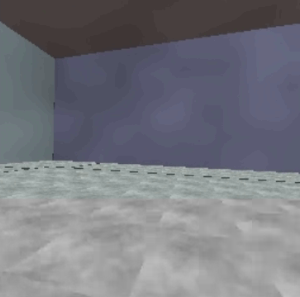
\includegraphics[width=20mm,height=14mm]{1.png}};
    \node[hotimageframe] (ftFrameTp1) at (7.8,4.9)
      {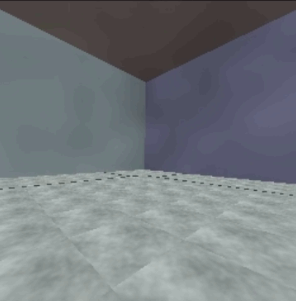
\includegraphics[width=20mm,height=14mm]{2.png}};
    \node[anchor=south east, font=\scriptsize] at (ftFrameT.north east) {$o_t$};
    \node[anchor=south east, font=\scriptsize] at (ftFrameTp1.north east) {$o_{t+1}$};
    \node[align=center, font=\scriptsize, text=ink!80] at (8,-7)
      {Real RGB\\observations \\ + unseen body};

    \node[align=center, font=\scriptsize, text=ink!85] (ftBodyLabel)
      at (14,35) {Body-motion label\\$\mathbf v_t$};
    \node[align=center, font=\scriptsize, text=ink!85] (ftActionLabel)
      at (14,-35) {Real joint command\\$a_t$};

    \coordinate (ftObsSplit) at (26,5);
    \draw[line] (ftFrameTp1.east) -- (ftObsSplit);
    \node[junction] at (ftObsSplit) {};
    \node[operation] (ftAugA) at (40,19) {Aug. $A$};
    \node[operation] (ftAugB) at (40,-9) {Aug. $B$};
    \draw[flow] (ftObsSplit) |- (ftAugA.west);
    \draw[flow] (ftObsSplit) |- (ftAugB.west);

    \node[encoder] (ftEncA) at (63,19) {Frozen Visual\\Encoder};
    \node[encoder] (ftEncB) at (63,-9) {Frozen Visual\\Encoder};
    \draw[flow] (ftAugA) -- (ftEncA);
    \draw[flow] (ftAugB) -- (ftEncB);
    \foreach \dy/\h in {-3/7,-1/11,1/9,3/13} {
      \fill[featureblue!82] (79+\dy,19-\h/2) rectangle ++(1.7,\h);
      \fill[featureblue!82] (79+\dy,-9-\h/2) rectangle ++(1.7,\h);
    }
    \coordinate (ftFeaturesA) at (86,19);
    \coordinate (ftFeaturesB) at (86,-9);
    \node[align=center, labelbox] (ftFeaturesALabel) at (80,11.5)
      {$(e_t^{A},e_{t+1}^{A})$};
    \node[align=center, labelbox] (ftFeaturesBLabel) at (80,-17)
      {$(e_t^{B},e_{t+1}^{B})$};
    \draw[flow] (ftEncA.east) -- (ftFeaturesA);
    \draw[flow] (ftEncB.east) -- (ftFeaturesB);
    \node[draw=ink!28, dashed, rounded corners=3pt,
      fit=(ftAugA)(ftAugB)(ftEncA)(ftEncB)(ftFeaturesALabel)(ftFeaturesBLabel),
      inner sep=4pt,
      label={[font=\scriptsize,text=ink!62]below:visual front-end; shared frozen encoder}]
      (ftVisualFrontend) {};

    \node[hotmodel] (ftItm) at (112,19)
      {Inverse Transition Model};
    \draw[flow] (ftFeaturesA) -- (ftItm.west);
    \node[steptag, anchor=south west] at (ftItm.north west) {1};

    \node[hotmodel, fill=latentfill, minimum width=25mm] (projector) at (112,-23)
      {Action Projector};
    \draw[target] (ftActionLabel.east) -- (90,-35) -- (90,-23) -- (projector.west);
    \node[steptag, anchor=south west] at (projector.north west) {2};

    \node[latent] (ftZ) at (140,1)
      {$z_t $\hspace{1.0mm}{\scriptsize\color{latentblue!85!black}$\in \mathbb{R}^{64}$}};
    \node[font=\scriptsize, text=ink!75, above=2.0mm of ftZ]
      {latent action};

    \draw[clearflow] (ftItm.south) -- (112,1) -- (ftZ.west);
    \draw[clearflow] (projector.north) -- (112,-2) -- (131.3,-2);

    \node[hotbodyhead] (ftBodyHead) at (180,21)
      {Body-motion Head};
    \node[hotmodel] (ftFtm) at (180,1)
      {Forward Transition Model};
    \node[decoder] (ftMd) at (180,-23)
      {Motion Decoder};
    \node[steptag, anchor=south west] at (ftFtm.north west) {1};
    \node[steptag, anchor=south west] at (ftBodyHead.north west) {3};
    \draw[clearflow] (ftZ.north) -- (140,21) -- (ftBodyHead.west);
    \draw[clearflow] (ftZ.east) -- (ftFtm.west);
    \draw[clearflow] (ftZ.south) -- (140,-20.2) -- ($(ftMd.west)+(0,2.8)$);

    \coordinate (ftContext) at (116,-9);
    \draw[line] (ftFeaturesB) -- node[above,labelbox] {$e_t^{B}$ context} (ftContext);
    \coordinate (ftCtxToFtm) at (180,-9);
    \draw[clearline] (ftContext) -- (ftCtxToFtm) -- (ftFtm.south);

    \node[loss] (ftBodyLoss) at (223,21) {$\mathcal L_{\mathrm{body}}$};
    \node[loss] (ftReconLoss) at (223,1) {$\mathcal L_{\mathrm{recon}}$};
    \node[loss] (ftMotionLoss) at (223,-23) {$\mathcal L_{\mathrm{motion}}$};
    \node[hotloss] (ftProjLoss) at (140,-41) {$\mathcal L_{\mathrm{proj}}$};
    \draw[flow] (ftBodyHead) -- node[above,labelbox] {$\hat{\mathbf v}_t$} (ftBodyLoss);
    \draw[flow] (ftFtm) -- node[above,labelbox] {$\hat e_{t+1}$} (ftReconLoss);
    \draw[flow] (ftMd) -- node[above,labelbox] {$\hat a_t$} (ftMotionLoss);
    \draw[clearflow] (projector.south) -- (112,-41) -- node[above,labelbox] {$\hat z_t$} (ftProjLoss.west);

    \draw[target] (ftBodyLabel.east) -- (223,35) --
      node[right,labelbox] {Froude $\mathbf v_t$} (ftBodyLoss.north);
    \draw[target] (86,-13) -- (223,-13) --
      node[pos=.65,right,labelbox] {$e_{t+1}^{B}$} (ftReconLoss.south);
    \draw[target] (ftActionLabel.east) -- (223,-35) --
      node[right,labelbox] {$a_t$} (ftMotionLoss.south);
  \end{scope}
\end{tikzpicture}%
}
\vspace*{\fill}
\end{document}
